\chapter{Teoretične osnove}

Parametre za iskano hidroelektrarno lahko izračunamo po naslednjem algoritmu:
\begin{enumerate}[noitemsep, topsep=0pt]
	\item Pridobitev podatkov
	\item Analiza hidrološkega niza podatkov za iskano obdobje
	\item Izračun konsumpcijske krivulje
	\item Izračun proizvodnje električne energije
\end{enumerate}


%-------------------------------------
\section{Pridobitev podatkov} \label{sec:teorija_pridobitevPodatkov}
Za nadaljnje izračune potrebujemo podatke o:
\begin{itemize}[noitemsep, topsep=0pt]
	\item Dimenzijah in naklonu rečne struge
	\item Manningovem koeficientu hrapavosti rečnega korita
	\item Povprečnih dnevnih pretokih vodotoka za izbrano obdobje
\end{itemize}

Podatke o dimenzijah rečnega korita lahko pridobimo z meritvami na terenu ali pa dimenzije ocenimo na podlagi ortofoto posnetkov. Naklon rečne struge vodotoka se lahko oceni s pomočjo spletne aplikacije Geopedija. Izberemo odsek vodotoka, ki ga definirata dve točki. S pomočjo Geopedije odčitamo podatke o višinski razliki $\Delta h$ in razdalji $\Delta L$ med točkama. S pomočjo spodnje enačbe določimo naklon izbranega odseka vodotoka:

\begin{ceqn}
\begin{align}
 I = \dfrac{100\Delta h}{\Delta L} [\%]
\end{align}
\end{ceqn}


  Manningov koeficient hrapavosti rečnega korita $ng$ se lahko oceni izkustveno na terenu s pomočjo priročnikov ali pa z umerjanjem na podlagi podatkov o nivojih vode in pretokih. Manningov koeficient hrapavosti je odvisen od naslednjih 7 faktorjev \cite{VenTeChow}:
 \begin{enumerate}[noitemsep, topsep=0pt]
 	\item Hrapavosti površine ostenja
 	\item Zaraščenosti rečnega korita
 	\item Neregularnosti oblike rečnega korita
 	\item Meandriranja rečne struge
 	\item Zamašitve struge s plavinami 
 	\item Oblike in velikosti rečnega korita
 	\item Polnosti rečnega korita z vodo
 \end{enumerate}
 

 
 
  Podatke o pretokih slovenskih vodotokov lahko pridobimo iz arhiva, ki se nahaja na spletni strani agencije Republike Slovenije za okolje (v nadaljevanju ARSO). V primeru da iščemo pretok za manjši vodotok, je zelo verjetno da podatki o pretokih vodotoka ne obstajajo. V tem primeru lahko pretok vodotoka ocenimo s pomočjo meritev višine gladine vode in dimenzij struge, ocene Manningovega koeficienta hrapavosti in naklona struge. S pomočjo Manningove enačbe opisane kasneje v poglavju~\ref{sec:teorija_trapeznaMetoda} in prej omenjenih členov Manningove enačbe dobimo končno ocenjeno vrednost pretoka vodotoka za posamezno obdobje meritev.




%------------------------------------------------
\section{Analiza hidrološkega niza podatkov}~\label{sec:teorija_hidrogramObdobja}
%TODO: FIXME -> izboljšaj
Iz ARSO-vega arhiva lahko izvozimo podatke o povprečnih dnevnih pretokih iskanega vodotoka v csv obliki (comma separated values). Iz izvoženih podatkov lahko za vsak mesec obdobja izračunamo povprečni mesečni pretok. Če mesečne pretoke povprečimo za vsa leta izbranega obdobja lahko navedene povprečne mesečne pretoke obdobja prikažemo na hidrogramu obdobja. Hidrogram je graf, ki prikazuje povprečne mesečne pretoke vodotoka za izbrano obdobje analize.  %Prav tako se lahko določi mokro in suho leto obdobja, ki ju primerjamo s povprečnimi mesečnimi pretoki.

%TODO: krivulja trajanja



%------------------------------------------------
\section{Izračun konsumpcijske krivulje}
Konsumpcijska krivulja je graf funkcije, ki predstavlja višino gladine vode v odvisnosti od pretoka vode v rečni strugi. Graf konsumpcijske krivulje potrebujemo za določitev višinske razlike $dh$ med spodnjo in zgornjo vodo hidroelektrarne v odvisnosti od pretoka vode skozi turbine hidroelektrarne. Višinsko razliko $dh$ potrebujemo za določitev moči hidroelektrarne v zadnjem koraku algoritma opisanega v tem poglavju.



%-------------------------------------------------
%TODO: opiši zakaj smo izbrali korak po cm
\subsection{Izračun konsumpcijske krivulje za pravokotne in trapezne struge} \label{sec:teorija_trapeznaMetoda}
Za izračun konsumpcijske krivulje potrebujemo pretok vodotoka $Q$ v odvisnosti od višine gladine vode $h$ v strugi. Gladina vode $h$ poteka od dna struge do maksimalne višine struge vodotoka $H$. Natančnost izračuna numeričnih metod, je odvisna od velikosti koraka izračuna. V našem primeru za potrebe ocene pretoka centimetrski korak po višini predstavlja zadostno natančnost. Pretok vode v strugi $Q$ se torej za vsak cm višine $h$ izračuna po Manningovi enačbi: 

\begin{ceqn}
\begin{align}
Q(h) = \dfrac{1}{ng} \sqrt{I}\dfrac{S(h)^{5/3}}{P(h)^{2/3}} \label{eq:ManningovaEnacba}
\end{align}
\end{ceqn}

Kjer je:

\begin{table}[htb!]
	\begin{tabular}{r|p{10cm}}
		Q & pretok \\
		ng & Manningov koeficient hrapavosti dna struge\\
		I & naklon struge \\
		S & ploščina omočenega dela prečnega profila \\
		P & dolžina omočenega oboda struge
	\end{tabular}
\end{table}


\newpage
% pravokotna struga
\begin{enumerate}
	\item Pravokotno oblikovana struga vodotoka:
	
	\begin{figure}[H]
		\begin{centering}
			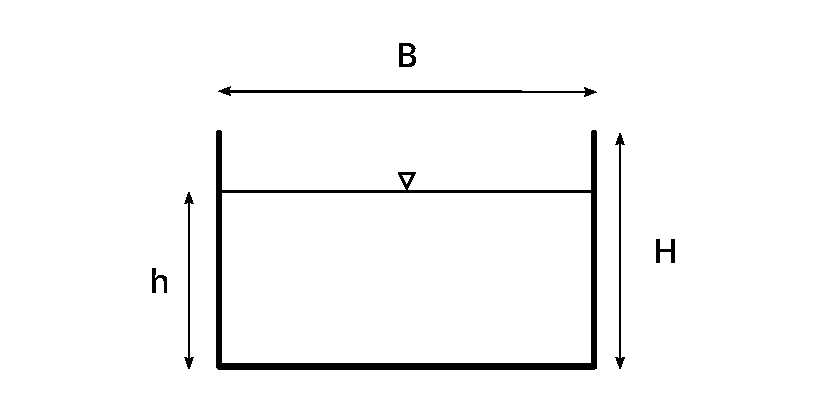
\includegraphics{slike/konsumpcijska_krivulja/rectangularChannel.pdf}		
			\caption{Prečni prerez pravokotne struge}\label{fig:pravokotna struga}
		\end{centering}
	\end{figure}
	

	Omočeni obod pravokotne struge izračunamo kot seštevek širine dna struge in dvakratne višine gladine vode v strugi vodotoka $h$.
	
	\begin{ceqn}
	\begin{equation}
	P_{p}(h) = B + 2h
	\end{equation}
	\end{ceqn}
	
	Ploščino omočenega dela, ki ga omejujejo rečno korito in gladina vode za pravokotno oblikovano rečno strugo dobimo po enačbi:
	
	\begin{ceqn}
	\begin{align}
	S_{p}(h) = B \cdot h
	\end{align}
	\end{ceqn}
	
	\item Trapezno oblikovana struga vodotoka:
	
		\begin{figure}[ht!]
			\begin{centering}
				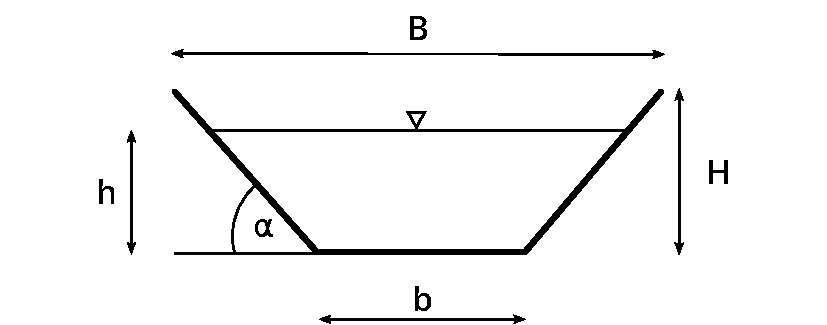
\includegraphics{slike/konsumpcijska_krivulja/trapezoidChannel.pdf}		
				\caption{Prečni prerez trapezne struge}\label{fig:trapezna struga}
			\end{centering}
		\end{figure}
	
	Omočeni obod trapezno oblikovane rečne struge izračunamo kot seštevek širine dna struge in dvakratne razdalje od roba dna do točke presečišča rečnega korita z gladino vode:
	
	\begin{ceqn}
	\begin{align}
	P_{t}(h) = b + 2 \cdot \sqrt{h^2 + \left(\dfrac{h} {\tan\alpha} \right)^{2}}
	\end{align}
	\end{ceqn}
	
	Ploščino omočenega dela v trapezno oblikovani rečni strugi izračunamo po enačbi:
	\begin{ceqn}
	\begin{align}
	S_{t}(h) = b \cdot h + \dfrac{h^2}{ 2\tan\alpha}
	\end{align}
	\end{ceqn}
	
\end{enumerate}



Ko poznamo vse parametre Manningove enačbe \ref{eq:ManningovaEnacba}, izračunamo pretoke vodotoka za vsak cm višine rečne struge, ki poteka od višine 0 do $H$ in narišemo graf konsumpcijske krivulje $h(Q)$.


\newpage
%------------------------------------------------
\subsection{Izračun konsumpcijske krivulje za struge poljubne oblike}\label{sec:pretokNumericnaMetoda}


V primeru, da iščemo konsumpcijsko krivuljo za strugo vodotoka poljubne oblike, si za izračun le te ne moremo pomagati s znanimi formulami preprostih geometrijskih likov. Poljubno oblikovano strugo lahko popišemo s serijo točk, ki jih dodajamo v kartezijski koordinatni sistem $x,y$. Za vsako točko ki definira poljubno rečno korito podamo x in y koordinato, za točke pa predpostavimo da so med seboj povezane z enačbo linearne funkcije. Na sliki~\ref{fig:poljubnaStruga} je predstavljen shema prečnega prereza poljubno oblikovane struge vodotoka.

\begin{figure}[ht!]
	\begin{centering}
		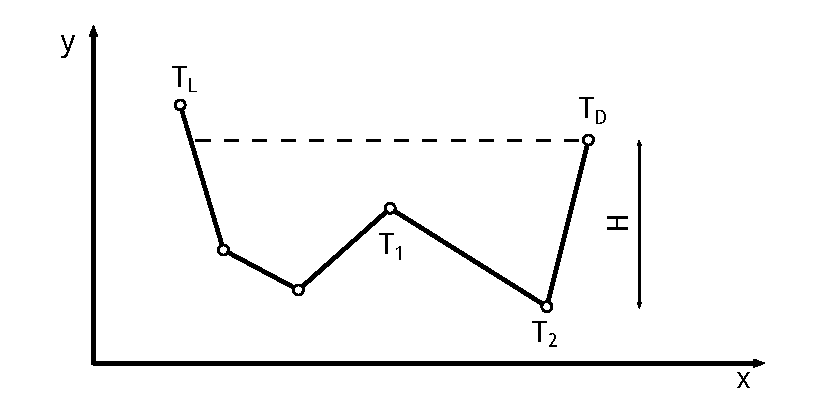
\includegraphics{slike/customChannel/customStruga.pdf}		
		\caption{Prečni prerez poljubno oblikovane struge vodotoka}\label{fig:poljubnaStruga}
	\end{centering}
\end{figure}



%------------------------------------------
%\subsection{Izračun višine rečnega korita}
Skrajni točki na robu struge vodotoka sta točki $T_L$ in $T_D$ na sliki \ref{fig:poljubnaStruga}. Točko na robu struge z nižjo y koordinato označimo s $T_{Rmin}$ (na sliki \ref{fig:poljubnaStruga} označena kot točka $T_D$). Najnižjo točko struge vodotoka označimo s $T_{min}$. Maksimalna višina gladine vode v rečnem koritu $H$ je definirana kot razdalja med točkama $T_{Rmin}$ in $T_{min}$. V primeru da je višina gladine vode večja od višine rečnega korita $H$ pride do preliva vode čez robove struge vodotoka.



%\subsection{Določitev parametrov odseka}
Za izračun konsumpcijske krivulje, s točkami definirano poljubno strugo vodotoka najprej razdelimo na odseke po dve točki $O_1$ ($x_1$, $y_1$) in $O_2$ ($x_2$, $y_2$) kar je prikazano na sliki \ref{fig:poljubnaStruga}. Za vsak analizirani odsek struge vodotoka, se najprej določi enačba linearne funkcije, ki povezuje točki $O_1$ in $O_2$.  Zaradi poenostavljenega zapisa so v nadaljevanju koordinate točke $O_1$ označene kot $x_1$ in $y_1$, koordinate točke $O_2$ pa $x_2$ in $y_2$.


Enačba linearne funkcije se definira kot:
\begin{ceqn}
\begin{align}
f(x) = kx + n \label{eq:enacba_linearnafunkcija}
\end{align}
\end{ceqn}

Naklon funkcije k se izračuna po spodnji enačbi:

\begin{ceqn}
\begin{align}
k = \dfrac{y_2 - y_1}{x_2 - x_1}
\end{align}
\end{ceqn}



Če v enačbo linearne funkcije \ref{eq:enacba_linearnafunkcija} vstavimo izračunan naklon $k$ in koordinate točke $O_1$, lahko izračunamo iskani $n$. S tem je določena enačba linearne funkcije $f(x)$ ki povezuje točki $O_1$ in $O_2$.

\begin{figure}[H]
	\begin{centering}
		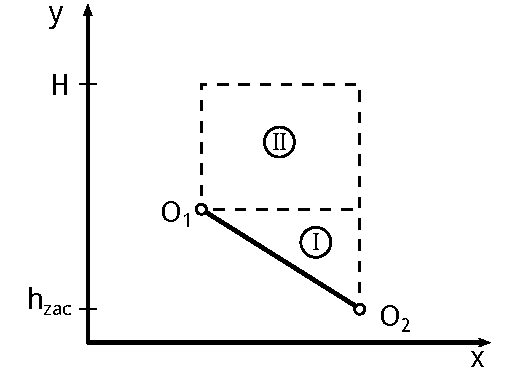
\includegraphics{slike/customChannel/odsek.pdf}
		\caption{Izbrani analizirani odsek struge} \label{fig:odsekStruge}
	\end{centering}
\end{figure}








% določitev ploščine posameznega kosa
Za vsak analizirani odsek dveh točk se določi najnižja točka odseka $T_z$, na sliki~\ref{fig:odsekStruge} označena kot točka $O_2$. Y koordinata točke $T_z$ nam predstavlja začetno višino odseka $h_{z}$. Od $h_z$ do končne višine gladine vode v strugi $H$ za vsak cm po višini določimo omočeni obod struge $P(h)$ in ploščino prečnega prereza odseka pod vodo $S(h)$. Razdaljo med $y$ koordinatami točk $O_1$ in $O_2$ označimo z $\Delta y$, razdaljo med $x$ koordinatami točk pa z $\Delta x$.  Ravnina $g$ predstavlja gladino vode pri trenutni višini $h$, kar je prikazano na sliki~\ref{fig:custom_odsekDetajl}.


\begin{figure}[ht!]
	\begin{centering}
		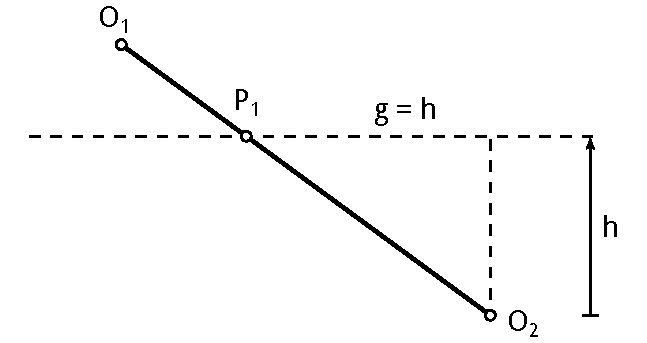
\includegraphics{slike/customChannel/odsek_detajl.pdf}
		\caption{Detajl izbranega odseka struge}\label{fig:custom_odsekDetajl}
	\end{centering}
\end{figure}



Omočeni obod struge vodotoka $P(h)$ in ploščina prečnega prereza struge vodotoka pod gladino vode $S(h)$ se glede na naklon funkcije, ki povezuje točki na robu analiziranega odseka $f(x)$ izračuna na dva načina:

\begin{enumerate}

\item V primeru ko velja $\Delta y = 0$ je funkcija med točkama odseka $f(x)$ vodoravna premica in velja:

\begin{ceqn}
\begin{align}
P(h)&= \Delta x\\
S(h)&= \Delta x \cdot h
\end{align}
\end{ceqn}


\item V primeru ko $\Delta y \neq 0$ ima funkcija $f(x)$ naklon $k \neq 0$. V tem primeru od začetka višine odseka $h_z$ do končne višine gladine vode v strugi $H$ za vsak cm izračunamo presečišče $G$, funkcije $f(x)$ s horizontalno ravnino $g = h$. 


Ko imamo določeno presečišče $G$ gladine vode s funkcijo $f(x)$ med točkama odseka, lahko izračunamo dolžino omočenega oboda struge odseka in ploščino lika ki ga oklepajo funkcija odseka $f(x)$, navidezna gladina vode $g = h$ in najnižja točka odseka $T_z$ (na sliki \ref{fig:odsekStruge} označena z $O_2$). 



Način izračuna omočenega oboda struge vodotoka $P(h)$ in ploščine prečnega prereza pod gladino vode $S(h)$ je odvisen od pozicije presečišča $G$:


\begin{enumerate}
	\item V primeru da se presečišče $G$ izbranega odseka struge nahaja v območju med točkama $O_1$ in $O_2$, dolžino omočenega oboda določimo po Pitagorovem izreku kot:
	
	%FIXME: decide on index G_x or Gx
	\begin{ceqn}
		\begin{align}
		P(h) = \sqrt{(T_{zx} - G_x(h))^{2} + (T_{zy} - G_y(h))^{2}}
		\end{align}
	\end{ceqn}
	
	
	Ploščino območja ki ga oklepajo horizontalna ravnina $g$ s presečiščem $G$ in najnižjo točko odseka $T_z$ pa določimo kot ploščino trikotnika (območje I na sliki~\ref{fig:odsekStruge}) po formuli:
	
	\begin{ceqn}
		\begin{align}
		S(h) = \dfrac{|T_{zx} - G_x(h)| \cdot |T_{zy} - G_y(h)|}{2}
		\end{align}
	\end{ceqn}
	
	
	\item V primeru, da se presečišče $G$ nahaja izven območja točk $O_1$ in $O_2$ se dolžina omočenega oboda odseka izračuna kot razdalja med točkama $O_1$ in $O_2$ po Pitagorovem izreku:
	
	\begin{ceqn}
		\begin{align}
		P = \sqrt{ \Delta x^{2} + \Delta y^{2}}
		\end{align}
	\end{ceqn}
	
	Ploščina pod gladino vode odseka $S(h)$ pa se določi kot seštevek ploščin območij I in II označenih na sliki \ref{fig:odsekStruge}.
	
	\begin{ceqn}
		\begin{align}
		S(h) = S_I + S_{II}(h)
		\end{align}
	\end{ceqn}
	
	Pri čemer sta $S_I$ in $S_{II}$ enaka:
	
		\begin{ceqn}
			\begin{align}
			S_I&= \bigg|\dfrac{ \Delta y \cdot  \Delta x}{2}\bigg|\\
			S_{II}(h)&= \bigg|\Delta x \cdot (h - y_1)\bigg|
			\end{align}
		\end{ceqn}
		
			
		
	\end{enumerate}
	
	





\end{enumerate}

%FIXME-URGENT -> Računanje S in P glede na pozicijo presečišča G








Ko imamo za vsak cm višine gladine vode izračunan omočeni obod $P_n(h)$ odseka $n$ in ploščino prečnega prereza pod gladino vode $S_n(h)$ lahko določimo pretok vode skozi odsek struge vodotoka $Q_n(h)$. Pretok vode skozi odsek izračunamo po Manningovi enačbi omenjeni v poglavju \ref{eq:ManningovaEnacba}. Za vsak računani odsek moramo poznati tudi naklon struge vodotoka $I_n$ in  Manningov koeficient hrapavosti površine $ng_n$, ki se ju določi po postopkih opisanih v poglavju \ref{sec:teorija_pridobitevPodatkov}.


\begin{ceqn}
	\begin{align}
	Q_n(h) = \dfrac{1}{ng_n} \sqrt{I_n}\dfrac{S_n(h)^{5/3}}{P_n(h)^{2/3}}
	\end{align}
\end{ceqn}


Posamezne pretoke odsekov po višinah medsebojno seštejemo in dobimo končne vrednosti pretokov $Q$ v odvisnosti od višine gladine vode v strugi vodotoka:

\begin{ceqn}
\begin{align}
Q(h) = Q_1(h) + Q_2(h) + Q_3(h) + ... + Q_{n-1}(h) + Q_n(h)
\end{align}
\end{ceqn}


S tem postopkom smo izračunali točke ki določajo konsumpcijsko krivuljo $h(Q)$ za izbrano strugo poljubne oblike.


\newpage

%TODO: dodaj Qtehnični, Qminimalni, kako se določi pretok skozi turbine.
\section{Izračun proizvodnje električne energije}
Za določitev končne proizvodnje električne energije potrebujemo razliko med koto zgornje vode t.j. vode v rezervoarju in koto spodnje vode t.j. vode ki teče skozi turbine hidroelektrarne. Ker računamo proizvodnjo električne energije za pretočne hidroelektrarne, predpostavimo da je kota zgornje vode konstantna na višini $H_z$.

\begin{figure}[ht!]
	\begin{centering}
		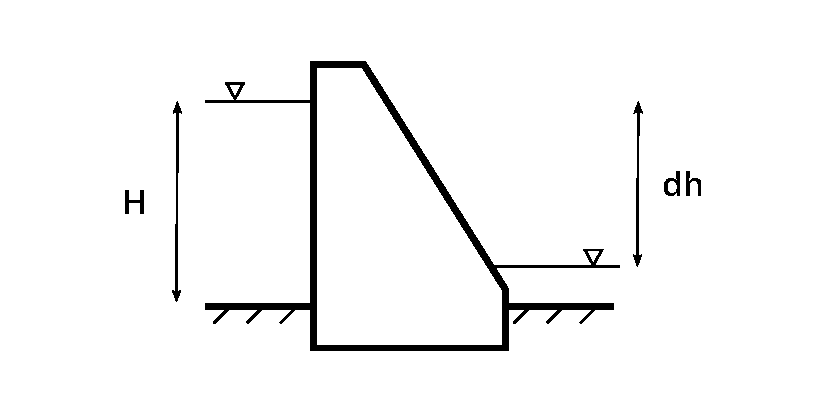
\includegraphics{slike/electricityProduction/powerplant_crossSection.pdf}
		\caption{Shema prečnega prereza hidroelektrarne}
	\end{centering}
\end{figure}

 Koto spodnje vode $H_s$ določimo iz prej izračunane konsumpcijske krivulje iz katere odčitamo višino gladine vode v strugi za dani povprečni mesečni pretok skozi turbine hidroelektrarne. V primeru da se pretok skozi turbine hidroelektrarne nahaja med dvema točkama pretokov v konsumpcijski krivulji, iskano višino spodnje vode določimo z linearno interpolacijo med znanima izračunanima točkama na grafu konsumpcijske krivulje.


Višinsko razliko med koto zgornje in spodnje vode določimo po spodnji enačbi:

\begin{ceqn}
\begin{align}
dh = H_z - H_s
\end{align}
\end{ceqn}

Moč hidroelektrarne izračunamo po enačbi:

\begin{ceqn}
\begin{align}
P = \eta \cdot \dfrac{g \cdot \rho_v}{1000} \cdot Q \cdot dh \label{eq:mocHidroelektrarne}
\end{align}
\end{ceqn}

Pri čemer so:
\begin{table}[htb!]
	\begin{tabular}{r|p{10cm}}
		P & moč [$kW$]\\
		$\eta$ & izkoristek turbine [\%]\\
		g & gravitacijska konstanta $\left[9,81~\dfrac{m}{s^{2}}\right]$ \\
		$\rho_v$&gostota vode $\left[\dfrac{1000 kg}{m^3}\right]$\\
		Q & pretok skozi turbine hidroelektrarne $\left[m^{3}/s \right]$\\
		dh & razlika višin spodnje in zgornje vode [$m$]
	\end{tabular}
\end{table}



Za ocenitev povprečne letne proizvodnje električne energije, potrebujemo podatke o povprečnih mesečnih pretokih vodotoka izračunanih za iskano časovno obdobje in parametrih turbin hidroelektrarne.

Za določitev pretoka skozi turbine hidroelektrarne potrebujemo osnovne podatke o hidroelektrarni, kot so minimalni pretok vode $Q_{min}$, maksimalni pretok $Q_{max}$ in tehnični maksimalni pretok hidroelektrarne $Q_{teh}$.

 Podatke o povprečnih mesečnih pretokih pridobimo iz rezultatov analize hidrološkega niza podatkov opisane v poglavju~\ref{sec:teorija_hidrogramObdobja}.






Za določitev povprečne mesečne proizvodnje električne energije potrebujemo znano povprečno mesečno moč hidroelektrarne  $\overline{P}$. Povprečno mesečno moč hidroelektrarne izračunamo s povprečjem dnevnih moči hidroelektrarne za iskani mesec. Za vsak mesec izračunamo povprečno moč hidroelektrarne po enačbi, pri čemer je $n$ število dni v mesecu:


\begin{ceqn}
\begin{align}
\overline{P} = \dfrac{P_1 + P_2 + P_3 + ... + P_{n-1} + P_n}{n}
\end{align}
\end{ceqn}



Povprečno mesečno proizvodnjo električne energije izračunamo po naslednji enačbi:

\begin{ceqn}
\begin{align}
E = \dfrac{24 \cdot \overline{P} \cdot d}{1000}
\end{align}
\end{ceqn}

Pri čemer so:
\begin{table}[htb!]
\begin{tabular}{r|p{10cm}}
	E & povprečna mesečna proizvedena električna energija [$MWh$]\\
	$\overline{P}$ & povprečna moč v mesecu [$kW$]\\
	d & število dni v mesecu \\
\end{tabular}
\end{table}


Končna povprečna letna proizvodnja električne energije je določena s seštevkom povprečnih mesečnih proizvodenj električne energije $E$:

\begin{ceqn}
\begin{align}
 E_{leto} =  \dfrac{E_1 + E_2 + E_3 + ... + E_{10} + E_{11} + E_{12}}{12} ~[MWh]
\end{align}
\end{ceqn}

